\section{Zielsetzung}
    \noindent In diesem Versuch soll der Photoeffekt untersucht werden. 
    Dabei soll insbesondere die Energie der aus einer Metallplatte ausgelösten Elektronen in Abhängigkeit von der dazu genutzten Photonenenergie untersucht werden.\\



\section{Theoretische Grundlagen}


    \noindent  Die Natur des Lichts lässt sich nicht klar dem Korpuskel- oder dem Wellenmodell zuordnen. 
    In der Quantenelektrodynamik allerdings sind diese beiden Fälle als Grenzfälle enthalten.\\
    Im folgenden Versuch wird bei der Erklärung auf das Korpuskelmodell zurückgegriffen.
    Da sich dieser Versuch nicht mit Licht als Welle erklären lässt hat er einen wesentlichen Teil dazu beigetragen, dass der Wellen-Teilchen-Dualismus des Lichts akzeptiert wurde.\\\\
    \noindent Bei diesem Versuch wird eine Metallplatte mit monochromatischem Licht bestrahlt. Dabei werden im besten Fall Elektronen aus der Platte gelöst.
    Um diese Elektronen messen zu können befindet sich gegenüber der einen eine weitere Platte, welche im Bezug zur ersten, ein positives Potential besitzt.\\
    Auf Grund des Potentialunterschieds beschleunigen sich dann die Elektronen von der ersten Platte, genannt Photokathode, zu der anderen Platte, genannt Auffängerelektrode.\\
    Dort ensteht dann an abfließender Strom, welcher mit einem Amperemeter gemessen werden kann.\\
    \noindent Schematisch dargestellt findet sich dieser Aufbau in der folgenden Abbildung \ref{img:schem}. 

    \begin{figure}[H]
        \centering
        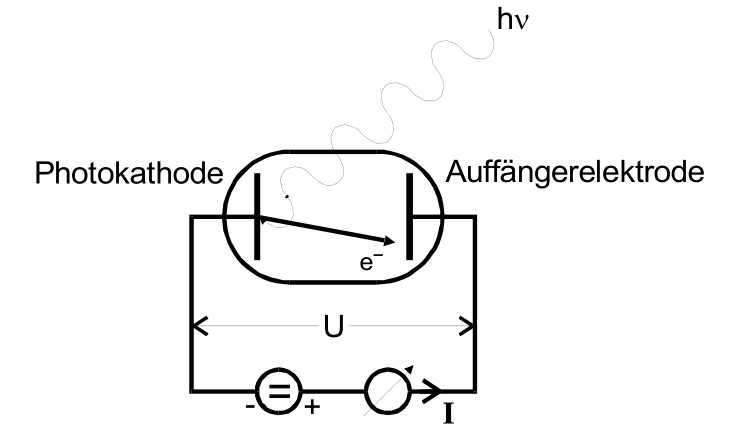
\includegraphics[width=0.75\textwidth]{latex/images/Schaltkreis.PNG}
        \caption{Der schematische Aufbau der zur Untersuchung des Photoeffekts dient\protect \cite{500}.}
        \label{img:schem}
    \end{figure}

    \noindent Für diesen Versuch gilt, dass die Anzahl der herausgelösten Elektronen proportional zur Intensität des Lichts, 
    die maximale kinetische Energie der Elektronen proportional zur Frequenz des Lichts und die Energie unabhängig von der Intensität ist.\\
    Zusätzlich existiert noch eine Grenzfrequenz des Lichts unterhalb welcher kein Effekt messbar ist.\\
    Dies sind alles Eigenschaften die sich nicht klassisch mit dem Wellenmodell nicht erklären lassen. Wenn aber nun angenommen wird, 
    dass sich die gesamte Energie in einem Teilchen mit praktisch verschwindender Ausdehnung konzentriert, lassen sich all diese Vorgänge erklären.
    Diese verschwindend kleinen Teilchen sind dann nach dem Korpuskelmodell die sogenannten Photonen.\\
    Sie haben die Energie $\symup{h}\cdot \nu$ wobei $\symup{h}$ das Planck'sche Wirkungsquantum\cite{Planck} ist.\\\\
    \noindent Hier übertragen dann, beim Auftreffen auf die Platte, die Photonen ihre Energie auf die Elektronen.
    Wenn die Energie des Photons groß genug ist um die materialabhängige Austrittsarbeit $A_K$ zu leisten verlässt das Elektron die Platte.
    Nun kann es mit der zuvor beschriebenen Methode detektiert werden.\\
    Wenn das Photon mehr Energie besitzt als für das Herauslösen benötigt wird erhält das Elektronen die Energiedifferenz als kinetische Energie.\\
    Es gilt also:
    \begin{equation*}
        \symup{h} \cdot \nu = E_{kin} + A_K
    \end{equation*}
    Außerdem folgt für die Grenzfrequenz, bei der $E_{kin}$ verschwindet:
    \begin{equation*}
        \nu=\frac{A_K}{\symup{h}}
    \end{equation*}
        
    \subsection{Die Photozelle}

    \noindent Der zuvor beschriebene Aufbau befindet sich in der Praxis in einem vakuumierten Glaskolben, welcher dann Photozelle genannt wird.\\
    In der Photozelle wird die Photokathode allerdings so realisiert, dass auf der Innenseite des Kolbens eine Metallschicht aufgedampft wird.
    Die Anode ist dann ein dazu parallel verlaufender Draht, der sich in kleinem Abstand dazu befindet.\\
    Dieser Aufbau ist in Abbildung \ref{img:schem} dargestellt.
    

    \begin{figure}[H]
        \centering
        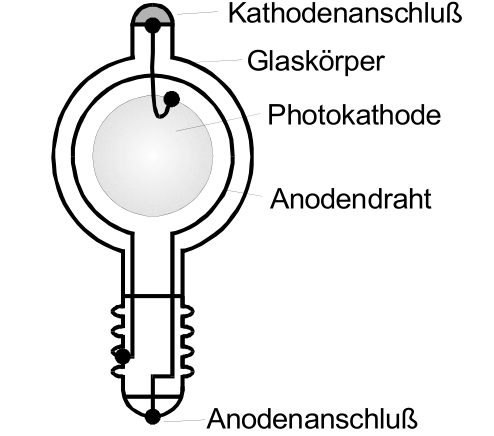
\includegraphics[width=0.35\textwidth]{latex/images/Photozelle.PNG}
        \caption{Der schematische Aufbau einer Photozelle wie sie in der Praxis verwendet wird\protect \cite{500}.}
        \label{img:schem}
    \end{figure}
    

    \noindent Anders als zuvor beschrieben wird hier an die Photzelle ein entgegengesetztes Feld angelegt.
    Dies ist die zur Untersuchung des Effektes genutzte, sogenannte Gegenfeldmethode.\\
    Die Elektronen werden weiterhin vom monochromatischen Licht herausgelöst müssen nun aber ein abbremsendes elektrisches Feld durchlaufen.
    Abhängig von der Anzahl der an der Anode gemessenen Elektronen und der angelegten Spannung lassen sich dann über die kinetische Energie 
    Rückschlüsse über die Geschwindkeitsverteilung der Elektronen schließen.\\
    Es können nun nämlich nur noch Elektronen die Anode erreichen deren kinetische Energie größer ist als $\symup{e_0} \cdot U$ mit $\symup{e_0}$ als Elementarladung\cite{e0}.\\
    Der Strom versiegt also bei
    \begin{equation*}
        \symup{e_0} \cdot U= \frac{\symup{m_0}\cdot v_{max}}{2}
    \end{equation*}
    Wobei $\symup{m_0}$ die Ruhemasse des Elektrons \cite{m0} und $v_{max}$ die Geschwindigkeit der schnellsten Elektronen ist.\\
    Daraus folgt wiederum für diese Elektronen:
    \begin{equation}
        \symup{h}\cdot \nu= \symup{e_0} \cdot U + A_K
        \label{eqn:vmax}
    \end{equation}


    \subsection{Die Geschwindigkeitsverteilung}


    Der in Gleichung \ref{eqn:vmax} beschriebene Zusammenhang gilt aber nur für die schnellsten Elektronen.
    Dies sind die Elektronen, welche schon in der Kathode die meiste kinetische Energie besitzen. 
    Dies führt dann für niedrigere Elektronen-Energien in der Kathode zu langsameren  Photoelektronen.\\
    Dies ist auch in der folgenden Grafik veranschaulicht, welche das mit steigender Bremsspannung kontinuierliche Abfallen der detektierten Photoelektronen zeigt.

    \begin{figure}[H]
        \centering
        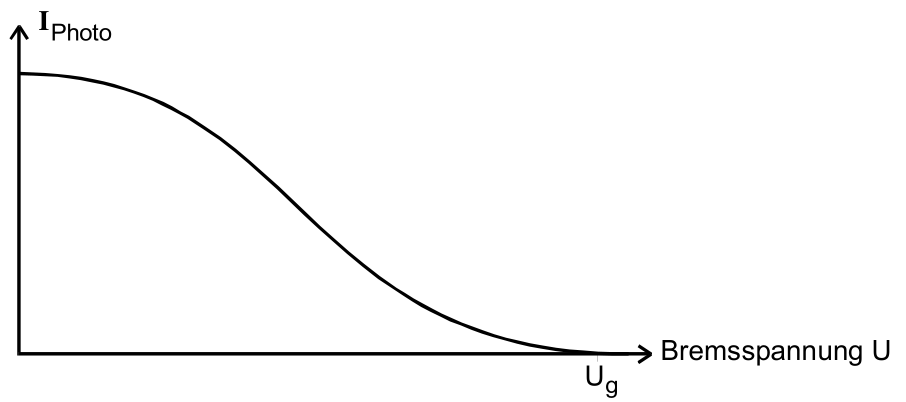
\includegraphics[width=0.7\textwidth]{latex/images/Bremsspannung.PNG}
        \caption{Das Abfallen des Photostroms mit steigender Bremsspannung qualitativ veranschaulicht \protect \cite{500}.}
        \label{img:brems}
    \end{figure}

    \noindent Die Energie der Elektronen in der Kathode lässt sich mit der Fermi-Dirac-Statistik beschreiben.\\
    Da diese aber hier nur begrenzt Gültigkeit besitzt, da nicht davon ausgegangen werden kann dass alle Photoelektronen die flächenmässig kleine Anode erreichen.
    Deswegen lässt sich einfach die folgende, hier gültige, quadratische Abhängigkeit der des Photostroms von der Spannung nutzen:
    \begin{equation}
        I_{ph} \sim U^2
        \label{eqn:quad}
    \end{equation}

    \noindent Die Fermi-Niveaus $\zeta$ von Metallen, die in der Fermi-Dirac-Statistik beschrieben sind aber trotzdem noch für diesen Versuch relevant.\\
    Denn wenn zwei unterschiedliche Metalle aneinander angeschlossen werden gleichen sich ihre Fermi-Niveaus auf die gleiche Höhe an.\\
    Dies kann dazu führen, dass wenn die Austrittsarbeit der Anode $A_A$ größer ist als die Energie der Photonen ist, kein Photoeffekt auftritt.
    Dies gilt auch dann wenn die Energie größer ist als $A_K$.
    Um dann einen Photstrom zu messen muss ein beschleunigendes Potential $U_b$ angelegt werden, so dass gilt:
    \begin{equation*}
        \symup{h} \cdot \nu + \symup{e_0} \cdot U_b \geq A_A
    \end{equation*}
    Auf Grund dieses Effekts lässt sich bei genügend großer Bremsspannung sogar ein entgegengesetzten Photostrom messen, welcher Messungen beeinträchtigen kann.







